% !Mode\dots ``TeX:UTF-8''
% !TEX root = ../root.tex
\section{Determining the online observability of \BCNs}
\label{sec:deter}
After defining the online observability and comparing it with the existing four observability, we propose two algorithms to determine the online observability of \BCNs. The first one is the supertree-based algorithm, and the second one is the algorithm based on directed graph. Based on the definition of online observability, we propose the supertree to describe the process of determining the initial state of a \BCN. And then, we propose the algorithm to determine the online observability of \BCNs\ based on the supertree. But the supertree-based algorithm can not help us find all paths to determine the initial state of some \BCNs. In order to improve the shortcomings of the supertree-based algorithm, we propose the algorithm based on directed graph. The algorithm based on directed graph may take longer time for us to determine online observability. But if we want do some optimizationin in the process of determining the initial state of a \BCN, this algorithm would be better. 
%And then, we analyze the complexity of the algorithm based on directed graph in this section. 
Finally, we represent how to determine the initial state of a \BCN\ by the directed graph.
%The construction processes of supertree and directed graph simulate derivation process of the initial state mentioned before. We check the super tree based on the definition of online observability of \BCNs\ depth first or breadth first. When we find enough leaf nodes, we can make sure the \BCN\ is online observable. But when we use the super tree to find all paths to determine the initial state of a \BCN, we need to check the existence of loops when we build the super tree. And many nodes in the tree are repeated, these nodes will take a lot of time overhead and space overhead for us to build and check the super tree for \BCNs. Therefore, we proposed the second way to determine the online observability of \BCNs\ by using directed graph. By this way we can avoid checking the existence of loop and avoid checking repeated nodes. There are also other advantages which help us select the input better in the process of determining the initial state of a \BCN\ by the second way. All of these advantages will reduce time and space overhead to determine the initial state of a \BCN. In conclusion if a \BCN\ seems to be online observable we would check it earlier by using supertree. But if a  \BCN\ does not seem to be online observable we prefer to check it earlier by using directed graph. If we just want to find a path to determine the initial state of a \BCN\ we would check it by using supertree. But if we want find all paths to determine the initial state of a \BCN\ and make some optimizations in the process of determine the initial state we prefer to check tthe \BCN\ by using directed graph.

\subsection{Supertree-based algorithm} %As we mentioned before, we can use the derivation function to determine the initial state of \BCNs. 
According to the definition of online observability, we alternately observe the output and decide the input in the process of determining the initial state of a \BCN. When the cardinal number of the set of possible states becomes $1$, we can determine the current state of this \BCN\ and then its initial state. Thus we define the supertree for \BCNs\ to describe this process, and propose the supertree-based algorithm to determine the online observability for \BCNs. For convenience, we use the set of states ($\mathsf{S}^i$) inside a node to represent this node, and the input ($\mathsf{i}^p$) or output ($\mathsf{o}^j$) in an edge to represent the edge.
\begin{definition}[Supertree]
For the supertree of a \BCN.   
\begin{itemize}
 \item  Every node of the supertree is labelled with a set of states ($\mathsf{S}^i$), and each edge is labelled with an input ($\mathsf{i}^p$) or output ($\mathsf{o}^j$).
 \item  The root node of the supertree is $\Delta_N$, and the leaf nodes of it are the nodes with cardinal number $1$.% ($|\mathsf{S}^i|=1$).
 \item In addition to the leaf nodes, 
 \begin{itemize}
 \item if a node $\mathsf{S}^i$ in the layer $2k + 1$ of the supertree, then for every $\mathsf{o}^j\in \Delta_Q$ if
\[|\Ded\left(\mathsf{S}^i,\varepsilon, \mathsf{o}^j\right)|>0,\]
 then $\Ded\left(\mathsf{S}^i,\varepsilon, \mathsf{o}^j\right)$ is one of the child nodes of $\mathsf{S}^i$, and $\mathsf{o}^j$ is the edge from $\mathsf{S}^i$ to $\Ded\left(\mathsf{S}^i,\varepsilon, \mathsf{o}^j\right)$.
 \item If a node $\mathsf{S}^i$ in the layer $2k+2$ of the supertree, then for each $\mathsf{i}^p \in \Delta_M$ if
\[|\Ded\left(\mathsf{S}^i,\mathsf{i}^p,\varepsilon\right)|=|\mathsf{S}^i|,\] 
then $\Ded\left(\mathsf{S}^i,\mathsf{i}^p,\varepsilon\right)$ is the child node of $\mathsf{S}^i$ and $\mathsf{i}^p$ is the edge from $\mathsf{S}^i$ to $\Ded\left(\mathsf{S}^i,\mathsf{i}^p,\varepsilon\right)$. 
 \end{itemize}
 
  
 \end{itemize}
\label{def:super-tree}
\end{definition}

  \begin{figure}[thpb]
      \centering
      \framebox{\parbox{3in}{
		\centerline{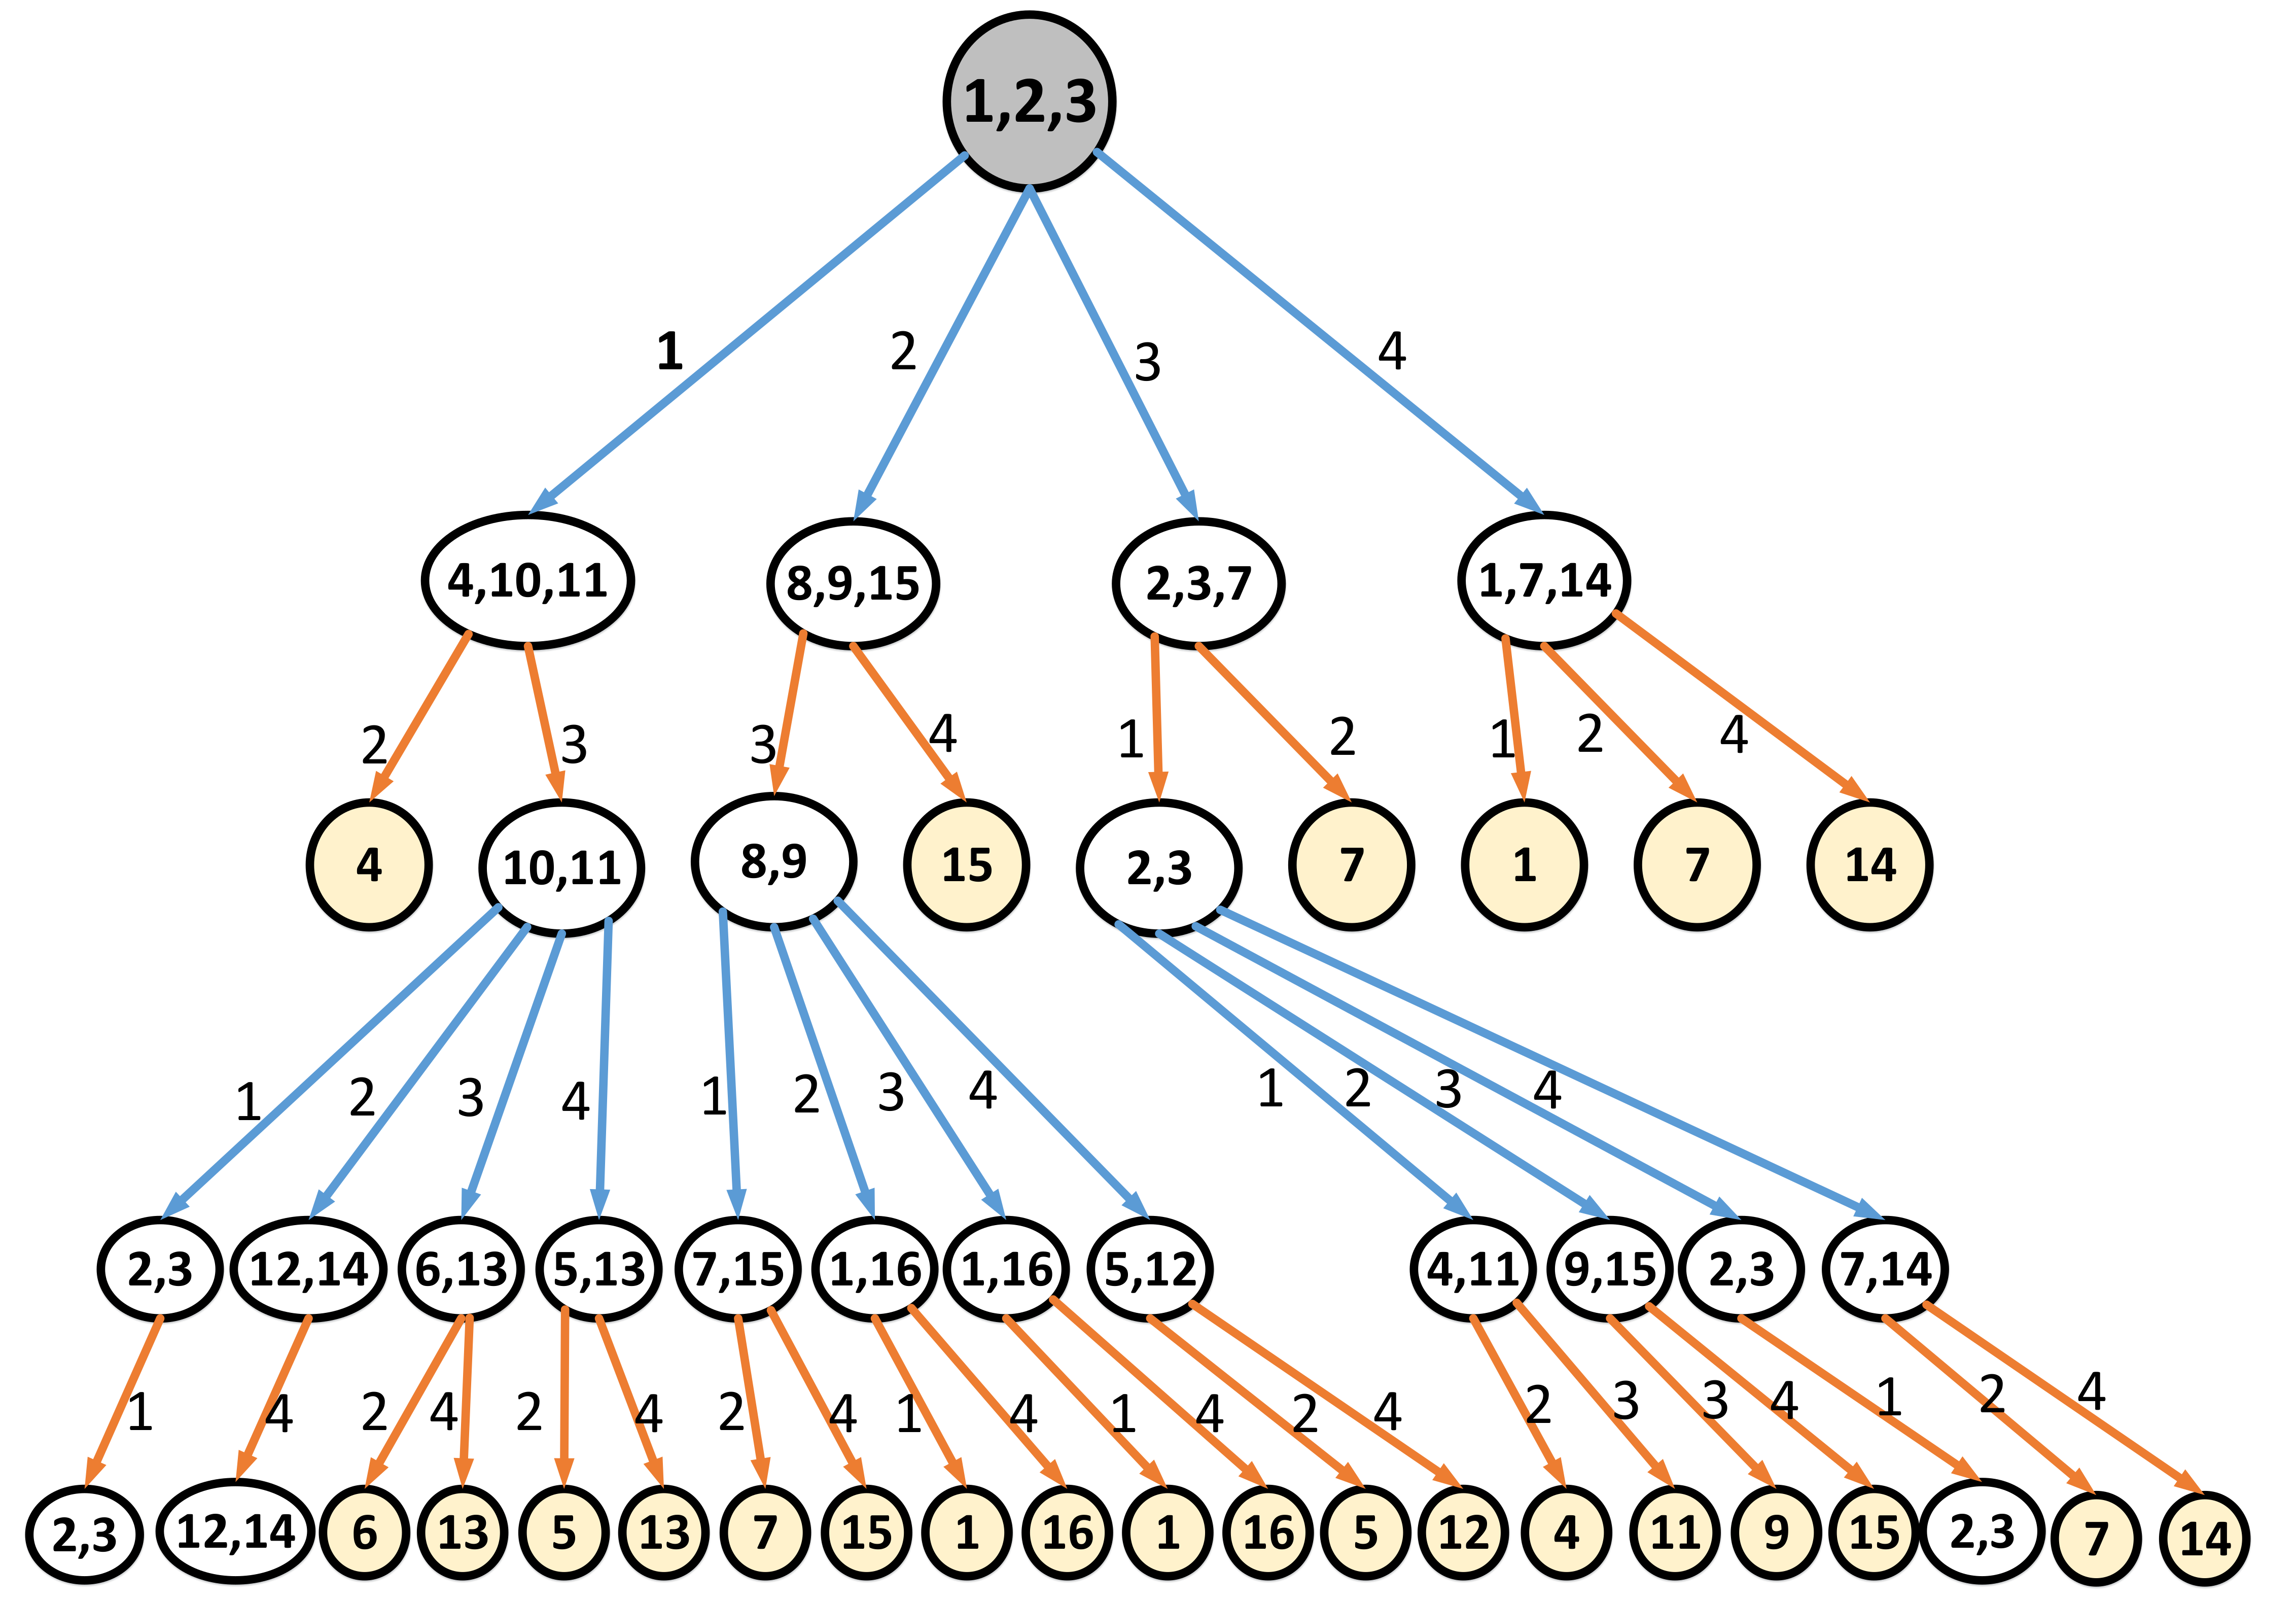
\includegraphics[scale=0.067]{figures/Fig3.png}}
	}}
      
      \caption{Branch of the super tree which represents $\{\delta_{16}^1,\delta_{16}^2,\delta_{16}^3\}$. The blue edges and orange edges show the observing output processes and deciding input processes, respectively. The yellow nodes are leaf nodes.}
      \label{fig:3}
   \end{figure}

As mentioned in the {\em Section \ref{sec:online}}, for a \BCN, we can only infer that the set of possible states is $\Delta_N$ at the beginning, thus the root node of super tree is $\Delta_N$. We can determine the state of the \BCN\ when the cardinal number of the possible states set becomes $1$. Therefore, the leaf nodes of supertree are the nodes with cadinal number $1$. In the process of determining the initial state of a \BCN, at every time step we observe the output $\mathsf{o}(t)$ of the \BCN\ to derive the set of possible states $\mathsf{S}(t)$ at first. After that, we derive and decide the input $\mathsf{i}(t)$ and then preliminarily derive the new possible states set of the \BCN. We alternately observe the output and decide the input untill we can determine the state of {\em BCN}. Therefore we use $\Ded\left(\mathsf{S}^i,\varepsilon, \mathsf{o}^j\right)$ to find child nodes for every $\mathsf{S}^i$ in $2k+1$ layer, and using $\Ded\left(\mathsf{S}^i,\mathsf{i}^p,\varepsilon\right)$ to find child nodes for every $\mathsf{S}^i$ in $2k+2$ layer. The formula 
\[|\Ded\left(\mathsf{S}^i,\varepsilon, \mathsf{o}^j\right)|>0\]
 ensures the node $\Ded\left(\mathsf{S}^i,\varepsilon, \mathsf{o}^j\right)$ is not empty. The formula 
 \[|\Ded\left(\mathsf{S}^i,\mathsf{i}^p,\varepsilon\right)|=|\mathsf{S}^i|\] 
 guarantee we can determine the state of \BCN\ in the end. Therefore, the paths to determine the initial state of a \BCN\ are described in the supertree, and then we can use the supertree to determine the online observability for a \BCN.

Based on the definition of the supertree, we propose the supertree-based algorithm ({\em Algorithm.\ref{alg:3}}) to determine the online observability for \BCNs. There are some details of {\em Algorithm.\ref{alg:3}} are as follows:
\begin{itemize}
\item In the supertree-based algorithm we build trees by breadth first. The $NodeArray$ and $NewArray$ represents the non-leaf nodes in layer $2k+1$ and $2k+2$ respectively. Then, the child nodes of $NodeArray$ are built by $\Ded\left(\mathsf{S}^i,\varepsilon, \mathsf{o}^j\right)$ and the child nodes of $NewArray$ are built by $\Ded\left(\mathsf{S}^i,\mathsf{i}^p,\varepsilon\right)$. And we use the $TemArray$ to store the child nodes of each in $NewArray$ or $NodesArray$.
\item We check the online observability of the \BCN\ by the definition of online observability and the supertree after $2k+2$ layer of the supertree was built for every $k\in  \mathbb{N}$. If the \BCN\ is online observable, then we stop building the supertree and delete the uncertain branches. 
\item Finally, we return the $\Delta_N$ which is the root node of the supertree, and then we can determine the initial state of the \BCN\ by the supertree.
 \end{itemize}
%If we want to find all of the ways to determine the initial state of a \BCN, we have to build all leaf nodes for the super tree of this \BCN. This process takes many additional time and space overhead. Especially when there are loops in the tree such as the $\{\delta_{16}^2,\delta_{16}^3\}$ in fourth layer and the $\{\delta_{16}^2,\delta_{16}^3\}$ in fifth layer which will form a loop. In this case we can never build the complete tree, thus we need to check the existence of loops and omit them. There are also some nodes take the same set of state, that they will take some additional overhead as well. For instance there are two nodes take the same states set $\{\delta_{16}^1,\delta_{16}^{16}\}$ in the fifth layer. However, using super tree would be a lot easier than using directed graph if we only need to find a way to determine the initial state. For instance, when we find the leaf nodes $\delta_{16}^1$, $\delta_{16}^7$ and  $\delta_{16}^{14}$ in third layer by breadth-first algorithm, we can make sure that the states set $\{\delta_{16}^1,\delta_{16}^2,\delta_{16}^3\}$ is 1 step deterministic. Therefore, we could use this conclusion to determine the initial state of this \BCN. 
\begin{algorithm}[h]
\caption{Supertree-based algorithm}
\begin{algorithmic}[1]
\REQUIRE 
The algebraic form of \BCN
\ENSURE  
The super tree of \BCN
\STATE  bool $Ob=$ false %(The online observability of \BCN)\
\STATE int $i$ \
\STATE int $j$ \
\STATE int $k$ \
%\STATE  $N_i$ (Node)\
%\STATE  $i_p$ (Input)\
\STATE node $NodeArray[N*M]$ %=$\Delta_N$\
\STATE  node $NewArray[N*M]$ %=$\Delta_N$\
\STATE  node $TemArray[M]$ %=$\Delta_N$\
\STATE $NodeArray[0]$ =$\Delta_N$\
%\STATE  $Sis$ (The suitable inputs set of $N_i$)\
%\STATE {\sf buildnode}(k)
%\STATE $k= k+1$
\WHILE {($Ob==$ false)}
\STATE  $j=0$ \
\FOR{($i=0$; $i<arraysize(NodeArray)$; $i++$)}
\STATE  $TemArray= $ Child nodes of $NodeArray[i]$ 
\FOR{($k=0$; $k<arraysize(TemArray)$; $k++$)}
\STATE$NewArray[j+k]=TemArray[k]$
\ENDFOR
\STATE$j=j+k$
\ENDFOR
\STATE Check this \BCN\ by the super tree
\IF{(\BCN\ is online observable)}
\STATE $Ob=$ true
\ELSE
\STATE  $i=0$ \
\FOR{($j=0$; $j<arraysize(NewArray)$; $j++$)}
\IF{(NewArray[j] is not leaf node)}
\STATE  $TemArray= $ Child nodes of $NewArray[j]$ 
\FOR{($k=0$; $k<arraysize(TemArray)$; $k++$)}
\STATE$NewArray[i+k]=TemArray[k]$
\ENDFOR
\STATE$i=i+k$
\ENDIF
\ENDFOR
\ENDIF
\ENDWHILE
\STATE Delete uncertain branches
%\STATE  $NodesArray$ =$\Delta_N$\
%\STATE return $Ob$
\STATE return $\Delta_N$\
\end{algorithmic}
 \label{alg:3}
\end{algorithm}

In order to better illustrate how to use the super tree to determine the online observability, we give the following example.
  
\begin{example}
For the \BCN\ mentioned in {\em Example \ref{exa:2}}. We need to determine for every \[\mathsf{o}^{j}(0)\in \Delta_Q\] such that \[|\Ded\left(\Delta_N,\varepsilon, \mathsf{o}^{j}(0)\right)|> 0,\] whether there exists a $k^{i}\in \mathbb{N}$ such that $\Ded\left(\Delta_N,\varepsilon,\mathsf{o}^{j}(0)\right)$ is $k^{i}$-step determinable.

Therefore, firstly we build child nodes for $\Delta_N$ by the $\Ded\left(\mathsf{S}^i,\varepsilon, \mathsf{o}^j\right)$ for every $\mathsf{o}^{j}(0)\in \Delta_Q$. For instance, \[\Ded\left(\Delta_N,\varepsilon,\delta_{4}^1\right)=\{\delta_{16}^1,\delta_{16}^2,\delta_{16}^3\}\] and we can not determine for $\{\delta_{16}^1,\delta_{16}^2,\delta_{16}^3\}$ whether there exists a $k^{i}\in \mathbb{N}$ such that $\{\delta_{16}^1,\delta_{16}^2,\delta_{16}^3\}$ is $k^{i}$-step determinable. Thus we can not determine the online observability of this \BCN\ by the supertree now. Therefore we build $2$ more layers for the \BCN\ as shown in the Fig.\ref{fig:3}. After that, as we check the second and third layer of this branch, we have the nodes $\{\delta_{16}^1\}$, $\{\delta_{16}^7\}$ and $\{\delta_{16}^{14}\}$ are $0$-step deterministic, and then we have the node $\{\delta_{16}^1,\delta_{16}^2,\delta_{16}^3\}$ is $1$-step deterministic. Using the same way to check other nodes, we can determine the online observability. Finally, we delete uncertain branches except the branches which can help us to determine online observability e.g. the first branch ($\{\delta_{16}^{4},\delta_{16}^{10},\delta_{16}^{11}\}$). Therefore, the supertree can help us to determine the initial state of the \BCN.%We can also determine the initial state of this \BCN\ by this branch.The nodes represent the sets of possible states, the blue edges represent the processes of observing output, and the orange edges represent the processes of deriving and deciding input. Only the yellow nodes are the leaf nodes, thus this branch is not completed. %When we check the second and third layer of this branch, we have the nodes $\{\delta_{16}^1\}$, $\{\delta_{16}^7\}$ and $\{\delta_{16}^{14}\}$ are $K$-step deterministic, and then we have the node $\{\delta_{16}^1,\delta_{16}^2,\delta_{16}^3\}$ is $K$-step deterministic. We can also determine the initial state of this \BCN\ by this branch.
\label{exa:11}
\end{example}   

However, if we want use the supertree-based algorithm to find all paths to determine the initial state of a \BCN\ we need to build all leaf nodes of its supertree. It would take many additional time and space overhead. Because 
\begin{itemize}
 \item there are many nodes with the same set of states in the supertree.
 \item And the same nodes in a path will form a loop, the loops in the supertree will prevent us from building a complete tree.
 \end{itemize}
For instance, in the Fig.\ref{fig:3} there are two nodes take $\{\delta_{16}^1,\delta_{16}^{16}\}$ in the fourth layer. And there are the $\{\delta_{16}^2,\delta_{16}^3\}$ in fourth layer and the $\{\delta_{16}^2,\delta_{16}^3\}$ in fifth layer would form a loop. With the shortcomings of the supertree, we propose the algorithm based on directed graph to help us find all paths to determine the initial state of a \BCN.
\subsection{Algorithm based on directed graph}
In order to improve the shortcomings of the supertree-based algorithm, we proposed the algorithm based on directed graph. The biggest difference between these two algorithms is the way the are constructed. The supertree is constructed from the root node ($\Delta_N$) to leaf nodes (contain 1 state), while the derected graph is constructed from smallest nodes (contain 1 state) to largest node (contain largest number of states). In addition, every node appears only once in the directed graph. What is more, the loops in the derected graph would not prevent us from building the directed graph completely.
Therefore, we have the definition of directed graph for \BCNs.
\begin{definition}[Directed Graph]
For the supertree of a \BCN.   
\begin{itemize}
\item Firstly, for every node $\mathsf{S}^i$ that $|\mathsf{S}^i|>1$, we have that for every distinct two $\mathsf{s}^a, \mathsf{s}^b \in \mathsf{S}^i$, $H\mathsf{s}^a=H\mathsf{s}^b$, and there are no duplicate nodes in the graph. 
\item Secondly, every node $\mathsf{S}^i$ in the directed graph there exists a $k^{i}\in \mathbb{N}$ such that $\mathsf{S}^i$ is $k^{i}$-step determinable. 

\item Finally, every edge of directed graph is labelled with an input ($\mathsf{i}^p$). 
\begin{itemize}
 \item If $|\mathsf{S}^i|=1$, then there are not edge from $\mathsf{S}^i$ to other nodes.
 \item  If $|\mathsf{S}^i|>1$, if for a $\mathsf{i}^p$ we have \[|\Ded\left(\mathsf{S}^i,\mathsf{i}^p,\varepsilon\right)|=|\mathsf{S}^i|.\] And every $\Ded\left(\mathsf{S}^i,\mathsf{i}^{p},\mathsf{o}^{j}\right)\ne\emptyset$ is a node of the graph, then there exists an edge each $\mathsf{i}^p$ from $\mathsf{S}^i$ to each $\Ded\left(\mathsf{S}^i,\mathsf{i}^{p},\mathsf{o}^{j}\right)$.
 
 %from it to one nodes, then there exist $z\ge 1$ such that there are $z$ edges contain $i_p$ from it to nodes $\mathsf{S}^1,\ldots,\mathsf{S}^z$ that \[|\mathsf{S}^i|= |\mathsf{S}^1|+,\ldots,|\mathsf{S}^z|\] and \[\Ded\left(\mathsf{S}^i,i_p,\varepsilon\right)=\mathsf{S}^1\vee,\ldots,\vee \mathsf{S}^z.\]
 \end{itemize}
 \end{itemize}
\end{definition}

From the {\em Lemma \ref{lemm:3}} in the {\em Section \ref{sec:online}}, we have that if for the set of states $\mathsf{S}^i$ there does not exist any $k^{i}\in \mathbb{N}$ such that $\mathsf{S}^{x}$ is $k^{i}$-step determinable, and $\mathsf{S}^{x}\subseteq \mathsf{S}^{y}$. Then there does not exist a $k^{j}\in \mathbb{N}$ that make $\mathsf{S}^{y}$ $k^{j}$-step determinable. Therefore, we check the $k$-step determinability of the nodes with fewer states at first, and then we check whether the nodes with more states in the process of building the directed graph for a \BCN. Once we can find that for a node $\mathsf{S}^i$ there does not exist any $k^{i}\in \mathbb{N}$ such that $\mathsf{S}^{i}$ is $k^{i}$-step determinable. Then we can make sure that there exists $\mathsf{o}^{j}\in \Delta_Q$ that $\mathsf{S}^{i}\subseteq \Ded\left(\Delta_N,\varepsilon, \mathsf{o}^{j}\right)$. Thus for $\Ded\left(\Delta_N,\varepsilon, \mathsf{o}^{j}\right)$ there does not exist any $k^{j}\in \mathbb{N}$ that make it $k^{j}$-step determinable either, and then this \BCN\ is not online observable. %Moreover, we can use the nodes with fewer states that are $k$-step deterministic to help us check the nodes with more states. For instance, if the node $S$ has two edges from it to two nodes $S_1$ and $S_2$, and we have $S_1$ and $S_2$ are $k$-step deterministic. In this case, we can make sure that the node $S$ is $k$-step deterministic.

With the definition of directed graph and the way to construct the derected graph. We propose the algorithm based on directed graph {\em Algorithm.\ref{alg:1}}, and the {\em Algorithm.\ref{alg:2}} to build nodes which is used in the {\em Algorithm.\ref{alg:1}}.

\begin{algorithm}[h]
\caption{Algorithm based on directed graph}
\begin{algorithmic}[1]
\REQUIRE 
The algebraic forms of \BCN
\ENSURE  
The directed graph of \BCN
\STATE bool $Ob=$ true %(The online observability of \BCN)\
\STATE int $i$ \
\STATE int $j$ \
\STATE int $k=1$ %(The number of states in the nodes)\
\STATE node $NodeArray[N*M]$
\STATE input $InputArray[M]$
%\STATE  $N_i$ %(Node)\
%\STATE  $i_p$ %(Input)\
%\STATE  $NodesArray$% (Nodes array)\
%\STATE  $Sis$ %(The suitable inputs set of $N_i$)\
\STATE {\sf buildnode}(k)
\STATE $k= k+1$
\STATE $NodeArray=${\sf buildnode}(k)
\WHILE {($NodeArray!=$Null)}
\FOR{($i=0$; $i<arraysize(NodeArray)$; $i++$)}
%\FOR{each $S_i\in NodesArray$}
\IF{($k==2$)}
\STATE $InputArray$ = $\Delta_M$ 
\ELSE

\STATE Find $InputArray$ by other nodes

\ENDIF
%\FOR{each $i_p \in Sis$}
\FOR{($j=0$; $j<arraysize(InputArray)$; $j++$)}
\STATE Check $NodeArray[i]$ by $InputArray[j]$ 
\STATE Build edges for $NodeArray[i]$ 
\ENDFOR
\IF {($NodeArray[i]$ has not any edge)}
\STATE  $Ob=$ false 
\STATE return Null
\ENDIF
\ENDFOR
\STATE $k= k+1$
\STATE $NodesArray=${\sf buildnode}(k)
\ENDWHILE
%\STATE $Ob=1$ 
%\STATE $NodesArray=${\sf buildnode}(k-1)
\STATE return $\Delta_N$\
\end{algorithmic}
 \label{alg:1}
\end{algorithm}
 %The algorithm to build nodes used in the Algorithm.\ref{alg:1} is shown in the Algorithm.\ref{alg:2}.
\begin{algorithm}[h!]
\caption{{\sf buildnode}(int k)}
\begin{algorithmic}[1]
\REQUIRE 
The number of states $k$
\ENSURE  
The nodes with $k$ states which with the same corresponding outputs %, and the outputs of $p$ states inside one node are the same.
%\STATE {\sf buildnode}(int p)
%\STATE  \{ 
%\dfSTATE $p=p+1$\
\STATE  Build all nodes with $p$ states %(whose outputs are the same)\

\IF{(Failed to build)} 
\STATE  return Null
\ELSE 
\STATE  Classify these nodes
\STATE Sort the states in these nodes
\STATE Sort these nodes%(For example, the nodes $\{\delta_{16}^1,\delta_{16}^2\}$, $\{\delta_{16}^1,\delta_{16}^3\}$ and $\{\delta_{16}^2,\delta_{16}^3\}$ shown in {\em Fig.\ref{fig:4}}. )
\STATE return nodes
\ENDIF 
%\STATE \}
\end{algorithmic}
 \label{alg:2}
\end{algorithm}
%%\newpage

There are some details in {\em Algorithm.\ref{alg:1}} and {\em Algorithm.\ref{alg:2}} are as follows:
\begin{itemize}
\item Build all nodes with $k$ states:
\begin{itemize}
\item Firstly, we classify all states by their corresponding outputs. Then we can get the set of states contains all states with the same corresponding outputs ($\Ded\left(\Delta_N,\varepsilon,\mathsf{o}^{j}\right)$).
\item Secondly, we compare $k$ with $|\Ded\left(\Delta_N,\varepsilon,\mathsf{o}^{j}\right)|$. If $k>|\Ded\left(\Delta_N,\varepsilon,\mathsf{o}^{j}\right)|$, then we could not get $k$ states from $\Ded\left(\Delta_N,\varepsilon,\mathsf{o}^{j}\right)$. Else we can get $C_{|\Ded\left(\Delta_N,\varepsilon,o_j\right)|}^k$ sets of states.
\item Finally, we use all of the sets of states found in second step to build nodes we need. 
\end{itemize} 
  %Finally, we use all of the sets of states found in second step to build nodes we need. 
 \item Sort the states in these nodes and sort these nodes: We sort the states inside the nodes at first, and then sort the nodes by the states of them. For example, the nodes $\{\delta_{16}^1,\delta_{16}^2\}$, $\{\delta_{16}^1,\delta_{16}^3\}$ and $\{\delta_{16}^2,\delta_{16}^3\}$ shown in Fig.\ref{fig:4}. 
  \item Find $InputArray$ by other nodes: From the {\em Lemma \ref{lemm:4}} in the {\em Section \ref{sec:online}}, we have if $\mathsf{S}^{x}\subset \mathsf{S}^{y}$ then for any input $\mathsf{i}^p\in \Delta_M$ for every $k^{i}\in \mathbb{N}$, if $\mathsf{i}^p$ can not make $\mathsf{S}^{x}$ $k^i$-step determinable, then it can not make $\mathsf{S}^{y}$ $k$-step determinable either. Therefor, for the node $NodeArray[i]$ contains $k$ sorted states, we can use the node with the first $(k-1)$ states of $\mathsf{S}^i$ and the node with the last $(k-1)$ states of $\mathsf{S}^i$ to find $InputArray$ for $NodeArray[i]$. For example, we can search the edges which from $\{\delta_{16}^4,\delta_{16}^5,\delta_{16}^6\}$ and $\{\delta_{16}^5,\delta_{16}^6,\delta_{16}^7\}$ at first. And then, take the intersection of this two sets of edges to be $InputArray$ of $\{\delta_{16}^4,\delta_{16}^5,\delta_{16}^6,\delta_{16}^7\}$. 
  \item Check $NodeArray[i]$ by $InputArray[j]$:
     
\begin{itemize}
\item If the input $InputArray[j]$ implies \[|\Ded\left(NodeArray[i],InputArray[j],\varepsilon\right)|<|NodeArray[i]|,\] then we can make sure the $InputArray[j]$ is a wrong input.
\item Else if every \[\Ded\left(NodeArray[i],InputArray[j],\mathsf{o}^{p}\right)\ne\emptyset\] already exists, then we contruct $NodeArray[i]$ if it does not exist in the graph, and connect it to $\Ded\left(NodeArray[i],InputArray[j],\mathsf{o}^{p}\right)$ with edge $InputArray[j]$.
\item Else if there exist a node \[\Ded\left(NodeArray[i],InputArray[j],\mathsf{o}^{p}\right)\] has not been constructed yet, then we check it latter. 
\end{itemize} 
\end{itemize} 

\begin{figure}[thpb]
      \centering
      \framebox{\parbox{3in}{
		\centerline{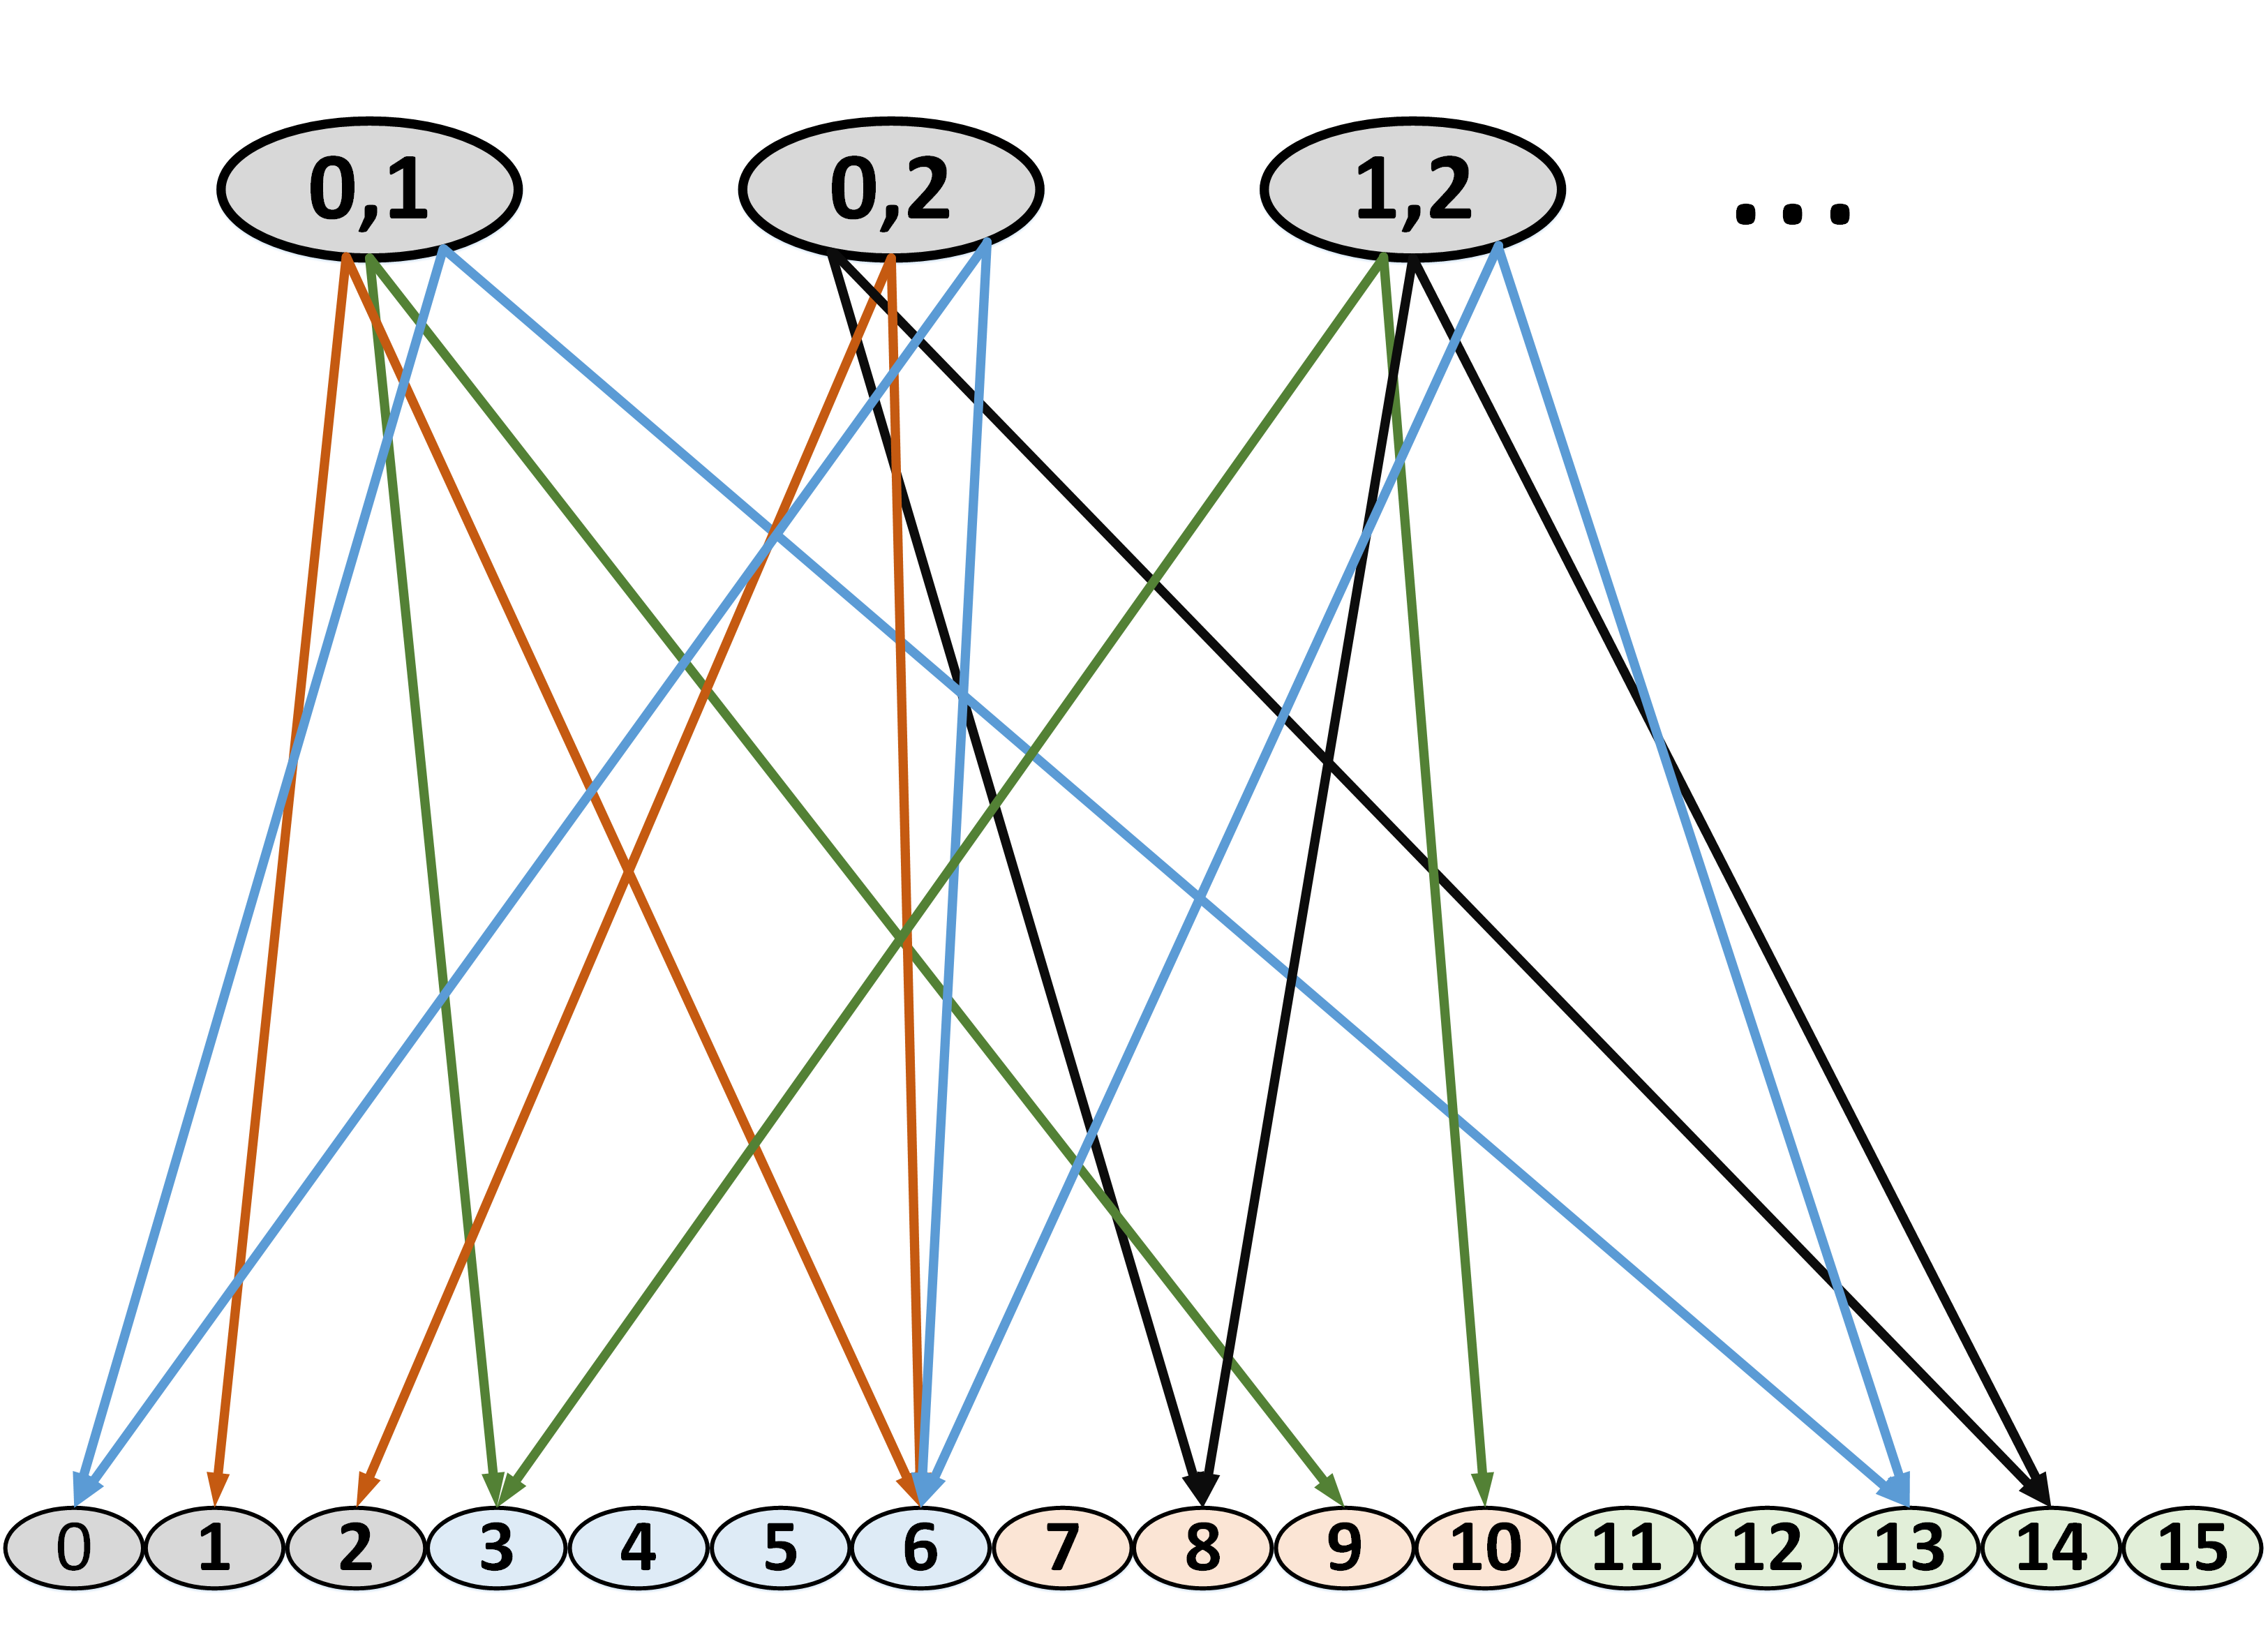
\includegraphics[scale=0.090]{figures/Fig4.png}}
	}}
      
      \caption{Part of the directed graph which represents $\{\delta_{16}^1,\delta_{16}^2\}$, $\{\delta_{16}^1,\delta_{16}^3\}$ and $\{\delta_{16}^2,\delta_{16}^3\}$. The green, black, orange, blue edges show the inputs $\delta_4^1$, $\delta_4^2$, $\delta_4^3$ and $\delta_4^4$ respectively.}
      \label{fig:4}
   \end{figure}

What is more, based on the definitions of existing four types of observability, we can also use the directed graph to determine the existing second and fourth type of observability for \BCNs. 
\begin{itemize}
 \item Checking the existing second observability: When we try to build bottom layer and penultimate layer of the directed graph, if some nodes in penultimate layer has no edges from it to other nodes. 
 Then, there are two distinct states $\mathsf{s}^x, \mathsf{s}^y \in \Delta_N$, $H\mathsf{s}^x=H\mathsf{s}^y$, such that for any $k\in \mathbb{Z}_+$ there does not exist any input sequence $\mathsf{I}\in(\Delta_M)^k$ implies $(HL)^k_{\mathsf{s}^x}(\mathsf{I})\neq (HL)^k_{\mathsf{s}^y}(\mathsf{I})$.
 And then, this \BCN\ does not satisfy existing second observability.
 \item  Checking the existing fourth observability: When we try to build the graph, if there exist one node with less than $\Delta_M$ edges, 
 then there exists an input sequence $\mathsf{I}\in(\Delta_M)^{\infty}$ does not satisfy for any distinct states $\mathsf{s}^x, \mathsf{s}^y \in \Delta_N$, $H\mathsf{s}^x=H\mathsf{s}^y$ implies $(HL)^{\infty}_{\mathsf{s}^x}(I)\neq (HL)^{\infty}_{\mathsf{s}^y}(I)$. And then this \BCN\ does not satisfy existing fourth observability.
 \end{itemize}

\begin{comment}

\subsection{Complexity analysis}
As the algorithm by the directed graph is better than by supertree when we want to find all paths to determine the initial state of \BCNs. We analyze the complexity of this algorithm briefly in this paper. 
%We classify the states with their corresponding output . After that form the set of states set $\{\Ded\left(\Delta_N,\varepsilon,\delta_M^1\right), \Ded\left(\Delta_N,\varepsilon,\delta_M^2\right),\ldots,\Ded\left(\Delta_N,\varepsilon,\delta_M^M\right)\}$, then every element in a states set has the same corresponding output. For each \[S_i\in\{\Ded\left(\Delta_N,\varepsilon,\delta_M^1\right), \Ded\left(\Delta_N,\varepsilon,\delta_M^2\right),\ldots,\Ded\left(\Delta_N,\varepsilon,\delta_M^M\right)\}\] we have $Hs_k=\delta_{M}^i$ for every $s_k\in S_i$.
\begin{itemize}
\item Firstly, we need to calculate the number of layers in the directed graph i.e. the upper bound of the number ($k$) of the states of the nodes in the directed graph. We have that 
\begin{equation}
\begin{split}
k_{upb}= \max(|\Ded\left(\Delta_N,\varepsilon,\delta_M^1\right)|,\ldots,|\Ded\left(\Delta_N,\varepsilon,\delta_M^M\right)|).
\end{split}
\end{equation}
%The upper bound of the number of the states of the nodes in the directed graph $k_{upb}$ is the maximum value of $|\Ded\left(\Delta_N,\varepsilon,\delta_M^1\right)|,\ldots,|\Ded\left(\Delta_N,\varepsilon,\delta_M^M\right)|$, 
Because the states of the same nodes in the directed graph should have the same corresponding output. Therefore, the $k_{upb}$ indicates the number of layers in the directed graph, and it depends on the relationship between states and outputs of the \BCNs.

\item Secondly, we need to calculate the number of nodes which with $k$ states, we have that
\begin{equation}
\begin{split}
Non(k)= C_{|S_i|}^k+\ldots +C_{|S_p|}^k,
\end{split}
\end{equation}
where \[S_i\ldots,S_p\in\{\Ded\left(\Delta_N,\varepsilon,\delta_M^1\right),\ldots,\Ded\left(\Delta_N,\varepsilon,\delta_M^M\right)\}\] and $|S_i|,\ldots,|S_p|\ge k$. The $Non(k)$ indicates the number of nodes which built by the {\sf buildnode}(k) function, and it also depends on the relationship between states and outputs of the \BCNs.

\item Thirdly, we need to calculate the cardinal number of suitable inputs set of each node $|Sis(S_i)|$. If $|S_i|=2$ then $Sis(S_i)=\Delta_M$. If $|S_i|>2$ then $Sis(S_i)$ is derived by other nodes, therefore it depends on the updating rules of the \BCNs.

\item Finally, we need to calculate the time used to check whether a input which in the suitable inputs set of a node is a right input for this node $T(S_i, i_p)$, and it depends on the updating rules of the \BCNs\ as well.
 \end{itemize}

After completing the previous analysis, we calculate the complexity by layer by layer, then we have the time we need to determine the online observability.  
\begin{equation}
\begin{split}
T=\sum_{k=1}^{k_{upg}}\sum_{i=1}^{Non(k)}\sum_{p=1}^{Sis(S_i)}T(S_i, i_p)
\end{split}
\end{equation}
%\[T=\sum_{k=1}^{k_{upg}}\sum_{i=1}^{Non(k)}\sum_{p=1}^{Sis(S_i)}T(S_i, i_p)\]
%The cardinal number of suitable inputs set of a node depends on the cardinal number of this node and the other three nodes used to find the suitable inputs set for it. And the time used to check whether an input is a right input for a node also depends on the updating rules of {\em BCNs}.

%What is more, instead of taking $\Delta_M$ as the suitable inputs set for every node in thedirected graph, we use the other three nodes like $\{\delta_{16}^4,\delta_{16}^5,\delta_{16}^6\}$, $\{\delta_{16}^5,\delta_{16}^6,\delta_{16}^7\}$ and $\{\delta_{16}^4,\delta_{16}^7\}$ that are $k$-step deterministic to find the suitable inputs set for a node $\{\delta_{16}^4,\delta_{16}^5,\delta_{16}^6,\delta_{16}^7\}$ which with more than $2$ states. By this way we can  reduce the cardinal number of the suitable inputs set for every nodes with more than 2 states, and then reduce the time cost. 

%The reason why we can use this method is that only the input which make the subset of $\{\delta_{16}^4,\delta_{16}^5,\delta_{16}^6,\delta_{16}^7\}$ $k$-step deterministic will make the $\{\delta_{16}^4,\delta_{16}^5,\delta_{16}^6,\delta_{16}^7\}$ $k$-step deterministic. Furthermore, using these three nodes will be a good way to cover all the 2-state subsets (which with cardinal number $2$) of $\{\delta_{16}^4,\delta_{16}^5,\delta_{16}^6,\delta_{16}^7\}$. For every subset $s_i$ with cardinal number $2$ included in $\{\delta_{16}^4,\delta_{16}^5,\delta_{16}^6,\delta_{16}^7\}$ will included in $\{\delta_{16}^4,\delta_{16}^5,\delta_{16}^6\}$, $\{\delta_{16}^5,\delta_{16}^6,\delta_{16}^7\}$ or $\{\delta_{16}^4,\delta_{16}^7\}$. This conclusion can help us to select the nodes we need when we seek the suitable inputs set for a node. But it is hard to analyze the complexity of this method, and it makes the complexity analysis of the algorithm by directed graph harder.

From the definition, we know that the $k_{upb}$ and the $Non(k)$ are depend on the relationship between states and outputs of the \BCNs, and the $|Sis(S_i)|$ and $T(S_i, i_p)$ are depend on the updating rules of the \BCNs. Therefore, it is hard to give an accurate complexity of the algorithm by the number of the nodes of the \BCNs\ without the complete imformation of their updating rules. We just give a brief introduction of complexity analysis in this paper, and we would do more research about this problem in the furture.
%Because the states in a nodes will have the same corresponding output, so we have the upper bound of the number of the states in a directed graph nodes $k$: We classify the states with their corresponding output and form the set of states with the same corresponding output, the greatest cardinal number of these set would be the upper bound of $k$. 

\end{comment}
\subsection{Determining initial state}

After introducing the algorithms to determine the online observability of the \BCNs, we present how to determine the initial state of a \BCN\ by the directed graph. In order to better illustrate the process of determining the initial state of a \BCN, we give one example is as follows.
\begin{example}
For the \BCN\ mentioned in {\em Example \ref{exa:2}}, the process of determining its initial state is shown in the Fig.\ref{fig:5}. 
\begin{itemize}
  \item Firstly, we observe the output of \BCN, if the output we observe $\mathsf{o}(0)=\delta_4^1$ then we can derive that the set of possible initial states $\mathsf{S}(0)=\{\delta_{16}^1,\delta_{16}^2,\delta_{16}^3\}$. Thus we record them as the initial states and current states of the \BCN\ in the table. 
  \item Secondly, we decide the input $\mathsf{i}(t-1)$ by $\mathsf{S}(t-1)$ and the directed graph, where $t>0$. With the $\mathsf{i}(t-1)$ and the output $\mathsf{o}(t)$ we observe, we can derive that the set of possible states $\mathsf{S}(t)$. And then we record them in their corresponding positions. 
 \item Repeating the second step untill the cardinal number of the set of possible states $|\mathsf{S}(t)|=1$. Then we can determine the state of \BCN\ $\mathsf{s}(t)=\delta_{16}^{6}$ and the corresponding initial state $\mathsf{s}(0)=\delta_{16}^{3}$.
\end{itemize} 
\end{example}   
%Input and output again and again 

\begin{figure}[thpb]
      \centering
      \framebox{\parbox{3in}{
		\centerline{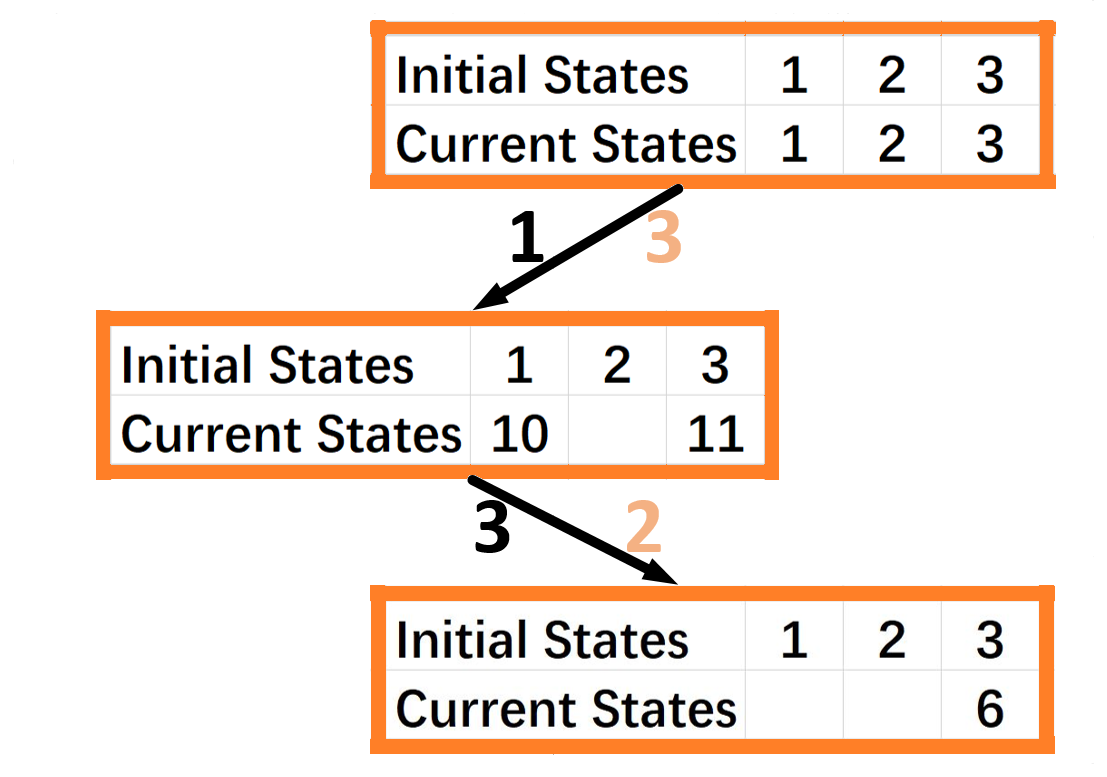
\includegraphics[scale=0.266]{figures/Fig5.png}}
	}}
      
      \caption{The process of determing the initial state of BCNs, we change the values of current states by input and the output we observe. }
      \label{fig:5}
   \end{figure}
%\subsection{Less observation costs}

Although the process of determining the initial state of a \BCN\ by the directed graph is very brief. But it would help us present how to do some optimization in the process of determining the initial state of the \BCNs.

